% 磁场中闭合电流的力矩

\pentry{安培力\upref{FAmp},力矩\upref{Torque}}
\begin{figure}[ht]
\centering
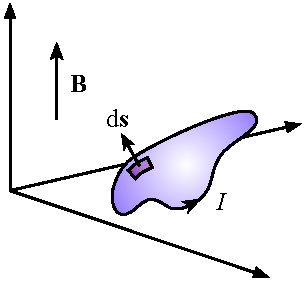
\includegraphics[width=5.5cm]{./figures/EBTorq1.pdf}
\caption{闭合电流在磁场中所受的力矩} \label{EBTorq_fig1}
\end{figure}
如\autoref{EBTorq_fig1}, 线圈中有闭合电流 $I$, 以及任意磁场分布 $\vec B(\vec r)$, 现在求线圈所受力矩.我们可以把线圈划分为许多小段 $\dd{\vec r}$,每小段的安培力产生的力矩为
\begin{equation}
\dd{\vec \tau} = \vec r\cross \dd{F} = \vec r \cross (I \dd{\vec r} \cross \vec B)
\end{equation}
对连续叉乘进行化简\upref{TriCro} 得
\begin{equation}
\begin{aligned}
\dd{\vec \tau} &=  \vec r \cross (I\dd{\vec r} \cross \vec B) =  I (\vec B \vdot \vec r) \dd{\vec r}  -  I\vec B (\vec r \vdot \dd{\vec r})
\end{aligned}
\end{equation}
对 $\vec r$ 沿闭合回路进行环积分得总力矩为
\begin{equation}
\begin{aligned}
\vec \tau & = \int \dd{\vec \tau} = I\oint (\vec B\vdot\vec r)\dd{\vec r}  - I\vec B\oint \vec r \vdot \dd{\vec r}
\end{aligned}
\end{equation}
其中
\begin{equation}
\oint \vec r \vdot \dd{\vec r}  = \oint r \uvec r \vdot \dd{\vec r}  = \oint r \dd{r}  = \eval{\frac{r^2}{2}}_{r_0}^{r_0}  = 0 % 未完成: 这个符号有介绍吗?
\end{equation}
这是因为换积分的起点和终点到原点的距离都相同. 所以
\begin{equation}\ali{
\vec \tau &= I \oint (\vec B \vdot \vec r) \dd{\vec r} \\
&= \uvec x I \oint (\vec B \vdot \vec r)\uvec x \vdot \dd{\vec r}  + \uvec y I \oint (\vec B \vdot \vec r)\uvec y \vdot \dd{\vec r}  + \uvec zI \oint (\vec B \vdot \vec r)\uvec z \vdot \dd{\vec r}
}\end{equation} 
对第一项进行分析,剩下两项类推即可
由斯托克斯定理得
\begin{equation}
\begin{aligned} 
\uvec x I \oint (\vec B \vdot \vec r)\uvec x \vdot \dd{\vec r}  &= \uvec x I \int \curl [ ( \vec B \vdot \vec r)\uvec x] \vdot \dd{\vec s} \\
&= \uvec x I \int \grad (\vec B \vdot \vec r) \cross \uvec x \vdot \dd{\vec s} \\
&= \uvec x I \int \dd{\vec s}  \cross \grad (\vec B \vdot \vec r) \vdot \uvec x 
\end{aligned} 
\end{equation}
其中面积分在以环路为边界的任意曲面进行.对 $\uvec y$ 和 $\uvec z$ 项也同样处理,得
\begin{equation}
\vec \tau = I \int \dd{\vec s}\cross\grad(\vec B\vdot\vec r)
\end{equation}
这是最一般的力矩表达式.

当磁场为匀强磁场时,由于 $\grad (\vec B \vdot \vec r) = \vec B$
\begin{equation}
\vec \tau = I \qty(\int \dd{\vec s}) \cross \vec B
\end{equation}







